\documentclass[12pt,a4paper]{article}
\usepackage[utf8]{inputenc}
\usepackage[russian]{babel}
\usepackage[OT1]{fontenc}
\usepackage{mathtools}
\usepackage{amsfonts}
\usepackage{amssymb}
\usepackage{enumitem}
\usepackage{alltt}
\usepackage{graphicx}
\usepackage{indentfirst}
\usepackage{caption}
\usepackage{float}
\usepackage{wrapfig}
\usepackage{physics}
\usepackage{multirow}
\usepackage{longtable}
\usepackage{amsmath,amsfonts,amssymb,amsthm,mathtools}
\usepackage{icomma}
\setlength{\parindent}{0.75cm}
\graphicspath{{pictures/}}
\DeclareGraphicsExtensions{.png, .jpg}
\usepackage[left=15mm,right=15mm,top=2cm,bottom=2cm]{geometry}
\author{Глотов Алексей}
\begin{document}
\newpage
\begin{center}
\footnotesize{{ГОСУДАРСТВЕННОЕ АВТОНОМНОЕ ОБРАЗОВАТЕЛЬНОЕ УЧРЕЖДЕНИЕ}\break
{ВЫСШЕГО ОБРАЗОВАНИЯ}
\break
{\bf {МОСКОВСКИЙ ФИЗИКО-ТЕХНИЧЕСКИЙ ИНСТИТУТ}}
\break
\small{(НАЦИОНАЛЬНЫЙ ИССЛЕДОВАТЕЛЬСКИЙ УНИВЕРСИТЕТ)}}
\break
\hfill \break
\hfill \break
\begin{center}
\normalsize{Кафедра общей физики}
\end{center}
\hfill \break
\hfill \break
\hfill \break
\hfill \break

\begin{center}
\normalsize {Лабораторная работа 5.2.2/5.2.3}
\end{center}
\hfill \break\\
\large{\textbf{Изучение спектров атомов водорода и молекулы йода}}
\end{center}
\begin{flushleft}
\hfill \break
\hfill \break
\hfill \break
\hfill \break
\hfill \break
\hfill \break
\hfill \break
\hfill \break
\hfill \break
\hfill \break
\hangindent=10cm
\normalsize{Преподаватель:} \;\;\;\;
\normalsize{к.ф.-м.н. Юрьев Ю.В.}\\
\hfill \break
\normalsize{Обучающийся:} \;\;\;\;\;
\normalsize{Глотов А.А} \\
\hfill \break
\end{flushleft}
\hfill \break
\hfill \break
\hfill \break
\hfill \break
\hfill \break
\hfill \break
\hfill \break
\hfill \break
\hfill \break
\hfill \break
\hfill \break

\begin{center}
Долгопрудный \break
 2023
\end{center}

\thispagestyle{empty}


\newpage
\section{Введение}

\subsection{Аннотация}

	Говорят, что атом водорода находится в возбуждённом состоянии, если его электрон находится не на основной орбитали. При смене своего энергетического уровня электрон поглощает/испускает энергия в виде фотона. Уровни энергий дискретны, поэтому и длины волн имеют строго определённые значения.
     Молекулы являются более сложными структурами, чем атомы. Помимо переходов электронов на более высокие орбиты в них может также происходить возбуждение колебательных и вращательных степеней свободы.

     \textbf{Цель:} Исследовать спектральные закономерности в оптическом спектре водорода. По результатам измерений вычислить постоянную Ридберга. Исследовать спектр поглощения паров йода в видимой области; по результатам измерения вычислить энергию колебательного кванта молекулы йода и энергию ее диссоциации в основном и возбужденном состояниях.
	


\subsection{Теоретические сведения}

Атом водорода является простейшей атомной системой; для него уравнение Шредингера можно решить точно. Решение примет вид:


\begin{equation}
E_n = - \frac{2\pi^2m_ee^4Z^2}{h^2}\frac{1}{n^2}
\end{equation}

А из формулы $(4)$ мы легко можем определить частоты излучения. 

Из рис.1 видно, что линии в спектре водорода можно расположить по сериям; для всех линий $n$ постоянно, а $m$ меняется от $n+1$ до $\infty$. 

В данной работе мы изучаем серию Бальмера, линии которой лежат в видимой области. 

Для серии Бальмера $n=2$, а $m = 3, 4, 5, 6$. Эти линии обозначаются $H_{\alpha}, H_{\beta}, H_{\gamma}, H_{\delta}$. Соответственные длины волн равны 656.3, 486.1, 434.1, 410.2 нм соответственно.

Рассмотрим структуру электронно-колебательного спектра поглощения молекулы йода. В зависимости от того, с какого колебательного уровня осуществляется переход можно выделить серии, начиная с нулевой. При этом из распределения Больцмана можно получить, что число молекул для этих серий можно соотносятся как :

$N_0 : N_1 : N_2 = 30 : 10 : 1$

Исходя из этого соотношения будем пренебрегать всеми сериями, кроме нулевой и первой.

     Обозначим энергию перехода с подуровня $n_1$ первого состояния на подуровень $n_2$ второго состояния как $h\nu_{n_1,n_2}$.
     
Имеем следующее соотношение:

\begin{large}
$h\nu_{n_1,n_2} = h\nu_\text{эл}+h\nu_2(n_2+1/2) - h\nu_1(n_1+1/2)$
\end{large}

\section{Результаты измерений и обработка данных}

Откалибруем монохроматор по известным спектральным линиям сначала неона, а потом ртути. По полученным данным построим график:

\begin{center}
\begin{tabular}{|c|c|c|c|c|c|c|c|c|c|c|c|c|c|}
\hline 
$\phi, ^\circ$ & 2536 & 2506 & 2442 & 2430 & 2400 & 2380 & 2370 & 2332 & 2326 & 2308 & 2296 & 2280  \\ 
\hline 
$\lambda$, нм & 703,2 & 692,9 & 671,7 & 667,8 & 659,9 & 653,3 & 650,7 & 640,2 & 638,3 & 633,4 & 630,5 & 626,7 \\ 
\hline 
$\phi, ^\circ$ & 2260 & 2238 & 2230 & 2208 & 2198 & 2178 & 2150 & 2138 & 2106 & 2092 & 1830 & 1792 & 1780 \\ 
\hline
$\lambda$, нм & 621,7 & 616,4 & 614,3 & 609,6 & 607,4 & 603,0 & 597,6 & 594,5 & 588,2 & 585,2 & 540,1 & 534,1 & 533,1  \\
\hline
\end{tabular} 
\end{center}

\begin{center}
\begin{tabular}{|c|c|c|c|c|c|c|c|c|c|}
\hline 
$\phi, ^\circ$ & 2550 & 2332 & 2120 & 2108 & 1930 & 1510 & 850 &  304   \\ 
\hline 
$\lambda$, нм & 690,7 & 623,4 & 579,1 & 577,0 & 546,1 & 491,6 & 435,8 & 404,1  \\ 
\hline 

\end{tabular} 
\end{center}

\begin{figure}[H]
	\begin{center}
		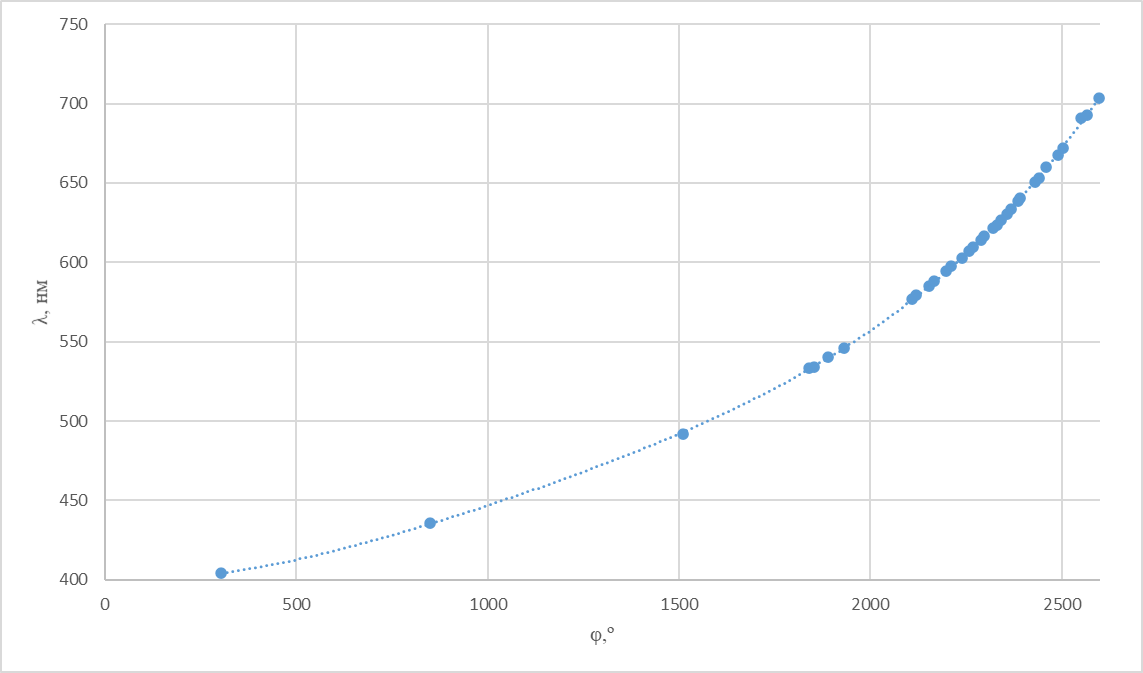
\includegraphics[width=14cm]{5.2.2-1}
		\caption{Калибровочный график}
	\end{center}
\end{figure}

По калибровочному графику (с помощью аппроксимационной кривой) определим значения длин вол серии Бальмера

\begin{center}
\begin{tabular}{|c|c|c|c|}
\hline 
 & $\phi, ^\circ$ & $\lambda$, нм & $\lambda_\text{теор}$, нм \\ 
\hline 
$H_\alpha$ & 2446 $\pm$2 & 656 $\pm$ 6 & 656.3 \\ 
\hline 
$H_\beta$ & 1454 $\pm$ 2 & 485 $\pm$ 4 & 486.1 \\ 
\hline 
$H_\gamma$ & 816 $\pm$ 2 & 438 $\pm$ 3 & 434.1 \\ 
\hline 
$H_\delta$ & 404 $\pm$ 2 & 410 $\pm$ 3 & 410.2 \\ 
\hline 
\end{tabular} 
\end{center}

Для определения постоянной Ридберга построим график зависимости

\begin{large}
$\frac{1}{\lambda}=f(\frac{1}{n^2} - \frac{1}{m^2} )$
\end{large}

\begin{figure}[H]
	\begin{center}
		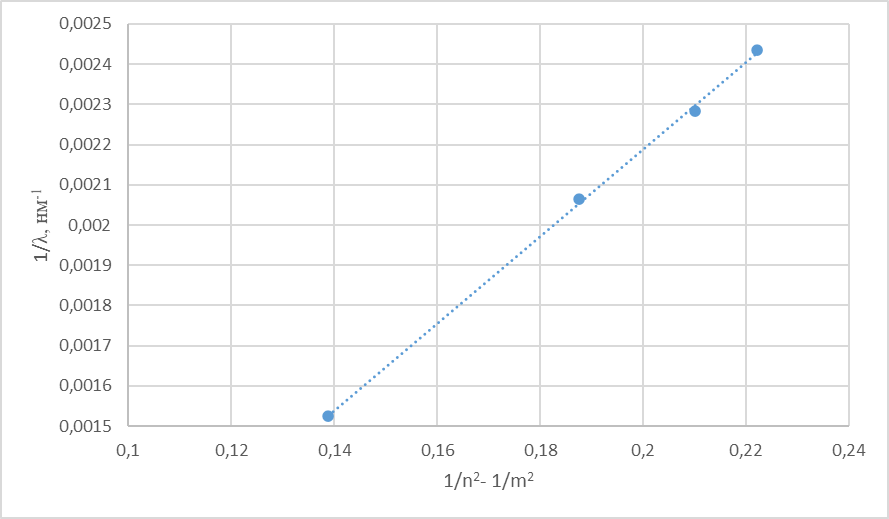
\includegraphics[width=14cm, height = 7cm]{5.2.2-2}
		\caption{Зависимость длины волны от номера перехода}
	\end{center}
\end{figure}

По МНК определим угловой коэффициент :

R = (0.011 $\pm$ 0.001) нм$^{-1}$

Визуально определим положение первой отчетливой линии поглощения (необходимости высматривать истинную первую линию нет необходимости - достаточное число линий в начале находятся на примерно одинаковом расстоянии). Затем визуально оценим границу сплошного поглощения

\begin{center}
\begin{tabular}{|c|c|c|c|}
\hline 
 & $h\nu_{1.0}$ & $h\nu_{1.5}$ & $h\nu_\text{гр}$ \\ 
\hline 
$\phi, ^\circ$ & 2248 $\pm$ 2 & 2148 $\pm$ 2 & 1650 $\pm$ 2 \\ 
\hline 
$\lambda$, нм & 606 $\pm$ 2 & 584 $\pm$ 2 & 505 $\pm$ 2 \\ 
\hline 
\end{tabular} 
\end{center}

\begin{large}
$h\nu_\text{гр} = \frac{hc}{\lambda_\text{гр}}$ = 2.45 $\pm$ 0.01 эВ
\end{large}

Энергия колебательного кванта возбуждённого состояния атома йода:

\begin{large}
$h\nu_2=\frac{h\nu_{1.5}-h\nu_{1.0}}{5}=\frac{hc}{5}\cdot(\frac{1}{\lambda_{1.5}} - \frac{1}{\lambda_{1.0}} = (0,015 \pm 0,001)$  эВ
\end{large}

	Энергия колебательного кванта в основном состоянии равна $h\nu_1$ = 0,027 эВ, энергия возбуждения атома $Е_{A}$ = 0,94 эВ. Определим энергия диссоциации молекулы в основном и возбуждённом состояниях, а также энергию электронного перехода:
    
\begin{large} 
$D_1 = (1,51 \pm 0,02)$  эВ

$h\nu_\text{эл} = (2,08 \pm 0,04)$  эВ

$D_2 = (0,40 \pm 0,03)$  эВ
\end{large}

\section{Обсуждение результатов и выводы}
	
  
     В ходе работы мы исследовали серию Бальмера в атоме водорода, определили постоянную Ридберга. Результат близок к теоретическому:
    
\begin{large}     
R=(0,108 $\pm$ 0,009)$\cdot 10^{-1} \text{нм}^{-1}$

$R_\text{теор} = 0,110 \cdot 10^{-1} \text{нм}^{-1}$
\end{large}

     Также мы определили энергии энергию электронного перехода между состояниями и энергии диссоциации молекулы $D_1$ в основном уровне и $D_2$ в возбуждённом состояниях.

\begin{large}
$D_1 = (1,51 \pm 0,02)$  эВ

$h\nu_\text{эл} = (2,08 \pm 0,04)$  эВ

$D_2 = (0,40 \pm 0,03)$  эВ
\end{large}

\end{document}